\chapter{Event generation, simulation and reconstruction}\label{ch:gensimreco}

\noindent The process of analyzing the data recorded by the CMS experiment involves several stages where the data are processed in order to interpret the information provided by all the detection systems; in those stages the particles produced after the \pp collision are identified by reconstructing their trajectories and measuring their features. In addition, the SM provides a set of predictions that have to be compared with the experimental results; however, in most of the cases, theoretical predictions are not directly comparable to experimental results due to the diverse source of uncertainties introduced by the experimental setup and theoretical approximations among others.\\

\noindent The strategy to face these conditions consist in using statistical methods implemented in computational algorithms to produce numerical results that can be contrasted with the experimental results. These computational algorithms are commonly known as Monte Carlo (MC) methods and, in the case of particle physics, they are designed to apply the SM rules and produce predictions about the physical observables measured in the experiments. Since particle physics is governed by quantum mechanics principles, predictions are not allowed for single events; therefore, a high number of events are ``generated'' and predictions are produced in the form of statistical distributions for the observables. Effects of the detector presence are included in the predictions by introducing simulations of the detector itself.\\     

\noindent This chapter presents a description of the event generation strategy and the tools used to perform the detector simulation and physics objects reconstruction. A comprehensive review on event generators for LHC physics can be found in reference \cite{gen} on which this chapter is based.  

\section{Event generation}

\begin{figure}[!h]
  \centering
  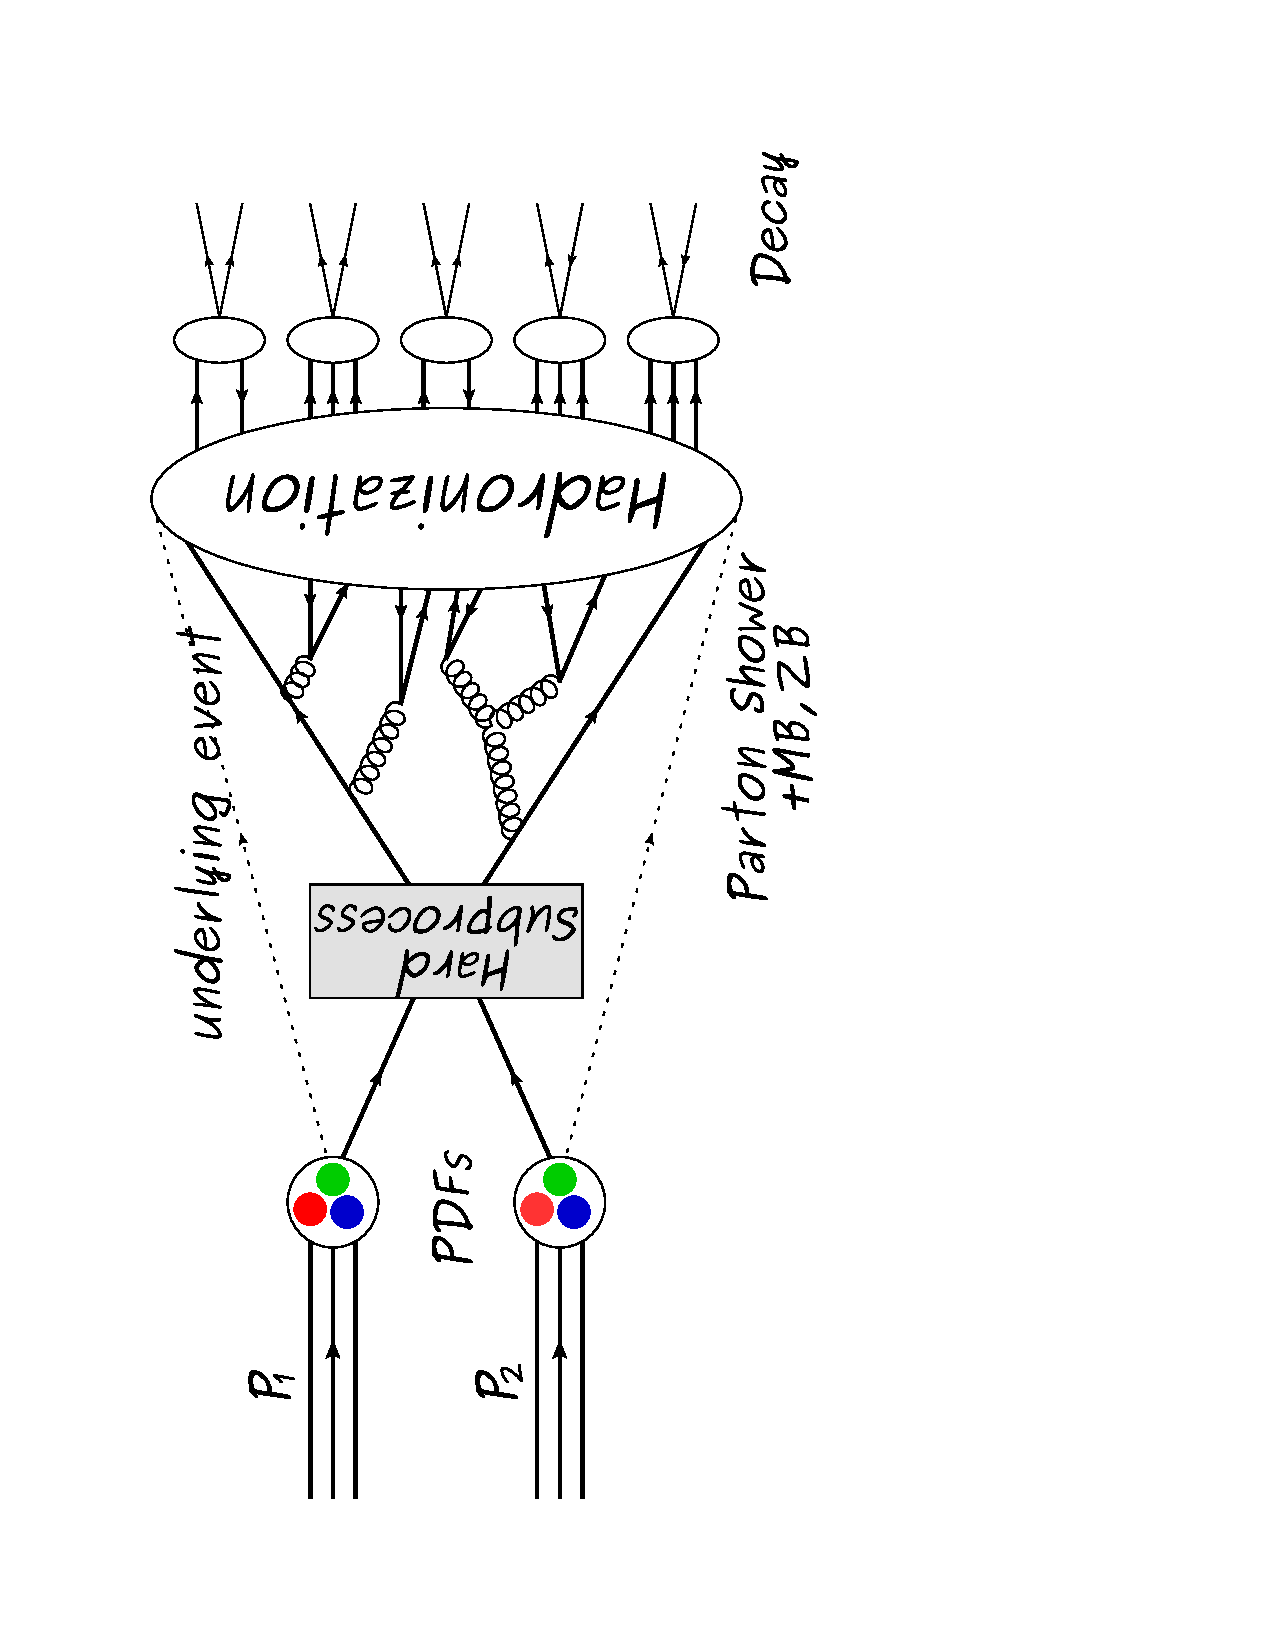
\includegraphics[scale=0.6,angle=-90]{gen}
  \caption[Event generation process.]{Event generation process. In the first step, the PDF of the colliding particles is considered so the specific interaction is described. The actual interaction is generated in the hard subprocess; the cross section of the process is calculated from the matrix element connecting the initial and final states. The parton shower describes the evolution of the partons from the hard subprocess according to the DGLAP equations. At this step the underlying event and PU efects are included in the generation. The resulting partons from the parton shower are recombined to form hadrons in the hadronization step; most of them are unstable, therefore, their decays are also generated in agreement to the known branching ratios. Modified from reference\cite{gen_scheme}.}\label{fig:gen}
\end{figure}

\noindent The event generation is intended to create events that mimic the behavior of actual events produced in the collisions; the obey a sequence of steps from the particles collision hard process to the decay process into the final state particles. Figure \ref{fig:gen} shows an schematic view of the event generation process; the fact that the full process can be treated as several independent steps is based on the QCD factorization theorem.\\     

\noindent Generation starts by taking into account the PDFs of the incoming particles. Event generators offer the option to chose from several PDF sets depending on the particular process under simulation\footnote{Tool in Reference \cite{pdfplot} allows to plot different PDF sets under customizable conditions.}; in the following \pp collisions will be considered. The \textit{hard subprocess} describes the actual interaction between partons from the incoming protons; it is represented by the matrix element connecting the initial and final states of the interaction. Normally, the matrix element can be written as a sum over Feynman diagrams and consider interferences between terms in the summation. During the generation of the hard subprocess, the production cross section is calculated. 

\noindent The order to which the cross section is calculated depends on the order of the Feynman diagrams involved in the calculation; therefore, radiative corrections are included by considering a higher order Feynman diagrams where QCD radiation dominates. Currently, cross sections calculated to LO do not offer a satisfactory description of the processes, \ie, the results are only reliable for the shape of distributions; therefore, NLO calculations have to be performed with the implication that the computing time needed is highly increased.\\       

\noindent The final parton content of the hard subprocess is subjected to the \textit{parton shower} which generates the gluon radiation. Parton shower evolves the partons; \ie, glouns split into quark-antiquark pairs and quarks of enough energy radiate gluons giving rise to further parton multiplication, following the DGLAP (Dokshitzer-Gribov-Lipatov-Altarelli-Parisi) equations. Showering continues until the energy scale is low enough to reach the non-perturbative limit.   

\noindent In the simulation of LHC processes that involve $b$ quarks like the single top quark or Higgs associated production, it is needed to consider that the $b$ quark is heavier that the proton; in this sense, the QCD interaction description is made in two different schemes \cite{schemes}

\begin{itemize}

\item four-flavor (4F) scheme. $b$ quarks appears only in the final state because they are heavier than the proton and therefore they can be produced only from the splitting of a gluon into pairs or singly in association with a $t$ quark in high energy-scale interactions. During the simulation, the $b$-PDFs are set to zero because it cannot be part of the proton. Calculation in this scheme are more complicated due to the presence of the second $b$ quark but the full kinematics is considered already at LO and therefore the accuracy of the description is better.   

\item five-flavor (5F) scheme. $b$ quarks are considered massless, therefore they can appear in both initial and final states since it can now be part of the proton; thus, during the simulation $b$-PDFs are not set to zero. In this scheme, calculations are simpler that in the 4F scheme and possible logarithmic divergences are absorbed by the PDFs through the DGLAP evolution.   
\end{itemize}

\noindent In this thesis, the \tHq events are generated using the 4F scheme in order to reduce uncertainties, while the \tHW events are generated using the 5F scheme to eliminate LO interference with the \ttH process\cite{demartin}.\\    

\noindent Partons involved in the \pp collision are the focus of the simulation, however, the rest of the partons inside the incoming protons are also affected because the remnants are colored objects; also, multiple parton interactions can occurs. The hadronization of the remnants and multiple parton interactions are known as ``underlying event'' and it has to be included in the simulation. In addition, multiple \pp collisions in the same bunch crossing (pile-up mentioned in \ref{sec:lhc}) occurs, actually in two forms

\begin{itemize}
\item \textit{in-time PU} which refers to multiple \pp collision in the bunch crossing but that are not considered as primary vertices. 
\item \textit{Out-of-time PU} which refers to overlapping \pp collisions from consecutive bunch crossings; this can occurs due to the time-delays in the detection systems where information from one bunch crossing is assigned to the next or previous one. 
\end{itemize}

\noindent While the underlying event effects are included in generation using generator-specific tools, PU effects are added to the generation by overlying Minimum-bias (MB) and Zero-bias (ZB) events to the generated events. MB events are inelastic events selected by using a loose (minimum bias) trigger with as little bias as possible, therefore accepting a large fraction of the overall inelastic event; ZB events correspond to random events recorded by the detector when collisions are likely. MB model in-time PU and ZB model out-of-time PU. 

\noindent The next step in the generation process is called ``hadronization''. Since particles with a net color charge are not allowed to exits isolated, they have recombine to form bound states. This is precisely the process by which the partons resulting from the parton shower arrange themselves as color singlets to form hadrons. At this step, the energy-scale is low and the strong coupling constant is large, therefore hadronization process is non-perturbative and phenomenological model are used to describe the parton's evolution. Most of the baryons and mesons produced in the hadronization are unstable and hence they will decay in the detector.\\

\noindent The last step in the generation process corresponds to the decay of the unstable particles generated during hadronization; it is also simulated in the hadronization step, based on the known branching ratios. 


\section{Monte Carlo Event Generators.}


\noindent The event generation described in the previous section has been implemented in several software packages for which a brief description is given.     

\begin{itemize}


\item rephare



  
\item MadGraph5\_aMC@NLO[83] is an next-to-leading order event generator including an optional parton shower step. It can calculate cross sections with full QCD corrections for a user given process, generate the hard process and is able to consistently match processes with radiations at tree-level with possible radiations of the parton shower. MadGraph5\_aMC@NLO was a merger of the two event generators MadGraph5 and aMC@NLO superseding both packages and is currently one of the most frequently used matrix element generators.
  
  A unique feature of MadGraph5\_aMC@NLO is the presence of negative event weights arising from the usage of counterterms that are needed to smoothen the phase space transitions between matrix element and parton shower dominated parts. Negative weights reduce the effective number of events that are used to reproduce object property shapes by filling histograms, which could lead to discontinuous shapes in exotic phase spaces with a low number of events.

Powheg Powheg[84–86], short for Positive Weight Hard Emission Generator, is an NLO matrixelement generator. Powheg models the hardest emission of color charged particles in an NLO process, making it necessary to interface it with a pT-ordered parton shower or a parton showerable to veto this highest emission, as else double counting of this highest-energetic emission would occur. This feature makes Pythia a natural match for the Powheg event generator.

\end{itemize}


MG5\_aMC@NLO (version 5.222)

pythia 8

madgraph

aC@NLO

powheg

MLM

CSV



%% MadEvent and M a d G ra p h
%% M a d E v e n t is a tree-level event generating software based on the matrix element generator
%% MadGraph, commonly only referred to as MadGraph [80, 81]. For a given process Mad -
%% Graph calculates the amplitudes for all contributing Feynman diagrams. This information can

%% then be evaluated by M a d E v e n t, which allows the user to calculate cross sections or decay
%% widths and produce unweighted events. MadGraph does not provide a parton shower and is
%% therefore often interfaced with P y t h i a.
%% Implemented in the MadGraph framework is the MadSpin [82] tool, which is used for the
%% decay of particles carrying non-zero spin.
%% Mad G ra p h 5 _ a M C @ N LO



%% Pyth i a
%% P y t h i a is a parton shower based multipurpose event generator. The calculation of the hard
%% matrix element is performed at leading order. The parton shower uses a p T -ordered emission
%% algorithm [87] and the Lund model for the hadronization.
%% Highly optimized parameter sets, known as tunes, are necessary to reproduce actual collisions
%% to a high degree of precision. The underlying event tune used in all samples for the analysis
%% √
%% √
%% at s = 8 TeV is the Tune Z2* [88], whereas in the analysis at s = 13 TeV the CUETP8M1
%% Tune [89] is employed in all samples.
%% In the Run I analysis of this thesis Pythia 6.4 [90] was used. During the first Long Shutdown
%% the new version P y t h i a 8 . 2 [91] was released and became the new standard in CMS for
%% parton showers.
%% As LO matrix-element generation is often not sufficient anymore, Pythia is often solely used
%% for the parton shower and is interfaced with other generators which take care of the matrix-
%% element generation.


%% Tauola
%% Due to the narrow width of the τ lepton its decay can be treated separately from its production.
%% In the Run I analysis the Tau o l a package [92] is applied, which only simulates the decay of
%% the τ lepton and has hence to be interfaced with other event generators. Spin effects as well as
%% electroweak corrections are taken into account by Tau o l a.









\noindent MC - MadEvent, MadGraph and madgraph\@NLO, powheg, pythia, tauola







\section{ detector simulation}

Monte Carlo Event samples will be generated to simulate the underlying physics collision.

The resulting particles will be tracked through the CMS detector and the electronics and trigger
responses will be simulated.

Both full and parametrized (fast) simulations will be required.

We anticipate using the full simulation package, OSCAR [4, 5], for most of these events.

Fully
simulated refers to detailed detector simulation based on GEANT4 [6], as opposed to faster
parametrized simulations. CMS has developed a fast simulation package, FAMOS [7], that may
be used where much larger statistics are required.

Fully simulated Monte Carlo samples of approximately the same total size as the raw data sample (1.5×109 events per year) must be generated, fully simulated, reconstructed and passed through HLT selection code. The simulated \pp event size is approximately 2 MByte/event.


We currently estimate that we will require the same order of magnitude of simulated events as actual data. If the Monte Carlo requirements greatly exceed this rough real data-sample equality, then more recourse to FAMOS will be necessary. Clearly there are very large uncertainties on the total amount of full and fast Monte Carlo which is required, so ultimately the reality of available resources will constrain the upper limit.




\section{event reconstruction- particle flow algorithm, vertexing , muon reco, electron reco, photon and hadron reco, jets reco, anti-kt algoritm, jet energy corrections, btagging, MET  }


CMS requires an offline first-pass full reconstruction of express line and all
online streams in quasi-realtime, which produces new reconstructed objects
called RECO data.


The Tier-0 offline reconstruction step processes all RAW events from the online system following
an adjustable set of priorities (the express-line, by definition has very high priority). This step
creates new higher-level physics objects such as tracks, vertices, and jets. These may improve or
extend the set produced in the HLT processing step. It must run with minimal delay compared
to the online in order to provide rapid feedback to the online operations, for example, identifying
detector or trigger problems which can then be rectified dynamically during the same LHC fill.
The offline reconstruction will normally perform the same reconstruction steps for each stream,
with the possible exception of specialised calibration streams. In this way we ensure that they
are all useful in principle for all analysis groups. We apply this same rule to later re-processings
of the data, 2-3 times per year we expect to bring all datasets into consistent status as to applied
calibrations and algorithms, as described below.





\section{ MVA methods, NN, BDT, boosting, overtraining, variable ranking  }
\section{statistical inference, likelihood parametrization}
\section{ nuisance paraeters}
\section{exclusion limits }
\section{asymptotic limits }












